\documentclass [xcolor=svgnames, t] {beamer} 
\usepackage[utf8]{inputenc}
\usepackage{booktabs, comment} 
\usepackage[absolute, overlay]{textpos} 
\usepackage{pgfpages}
\usepackage[font=footnotesize]{caption}
\useoutertheme{infolines} 



%\definecolor{brownbrown}{RGB}{56, 28, 0}
%\definecolor{brownred}{RGB}{228, 0, 43}

%\setbeamercolor{title in head/foot}{bg=brownred, fg=brownbrown}
%\setbeamercolor{author in head/foot}{bg=myuniversity}
\setbeamertemplate{page number in head/foot}{}
\usepackage{csquotes}


\usepackage{amsmath}
\usepackage[makeroom]{cancel}


\usepackage{textpos}

\usepackage{tikz}

\usetheme{Madrid}
%\definecolor{myuniversity}{RGB}{56, 28, 0}
%\usecolortheme[named=myuniversity]{structure}

\title[Introducci\'on]{Clase No.03: Introducci\'on}
\subtitle{Planteamiento del problema o idea a desarrollar}
\institute[]{Departamento de Ingenier\'ia Civil y Agr\'icola\\ Facultad de Ingenier\'ia  \\Universidad Nacional de Colombia - Sede Bogot\'a}
\titlegraphic{
\includegraphics[height=2.0cm]{escudoUnal.png}}
\author[LAM]{Luis Alejandro Morales \\ \href{https://lamhydro.github.io}{https://lamhydro.github.io}}
%\date{\today}
\date{}


\addtobeamertemplate{navigation symbols}{}{%
    \usebeamerfont{footline}%
    \usebeamercolor[fg]{footline}%
    \hspace{1em}%
    \insertframenumber/\inserttotalframenumber
}

\begin{document}
\begin{frame}
\maketitle
\end{frame}


%%%%%%%%%%%%%%%%%%%%%%%%%%%%
\logo{\vspace{-0.2cm}
\includegraphics[height=0.8cm]{escudoUnal.png}~%
}
%%%%%%%%%%%%%%%%%%%%%%%%%%



\begin{frame}
\frametitle{Table of Contents}
\tableofcontents
\end{frame}

%%%%%%%%
\section{¿Que es un problema o idea de investigaci\'on o profundizaci\'on?}

\begin{frame}{Problema o idea de investigaci\'on o profundizaci\'on}
\begin{columns}
\column{0.5\textwidth}
\begin{exampleblock}{Idea de investigaci\'on o profundizaci\'on}
\begin{itemize}
\item Sugiere la posibilidad de hacer un estudio.
\item Surge de la observaci\'on de un problema o la detecci\'on de una brecha en el conocimiento. O del inter\'es de explorar un aspecto de alguna disciplina.
\item Proporciona el punto de partida para la generaci\'on de preguntas e hip\'otesis de investigaci\'on.
\item A partir de la idea se formula un proyecto de investigaci\'on.
\end{itemize}
\end{exampleblock}
\column{0.4\textwidth}
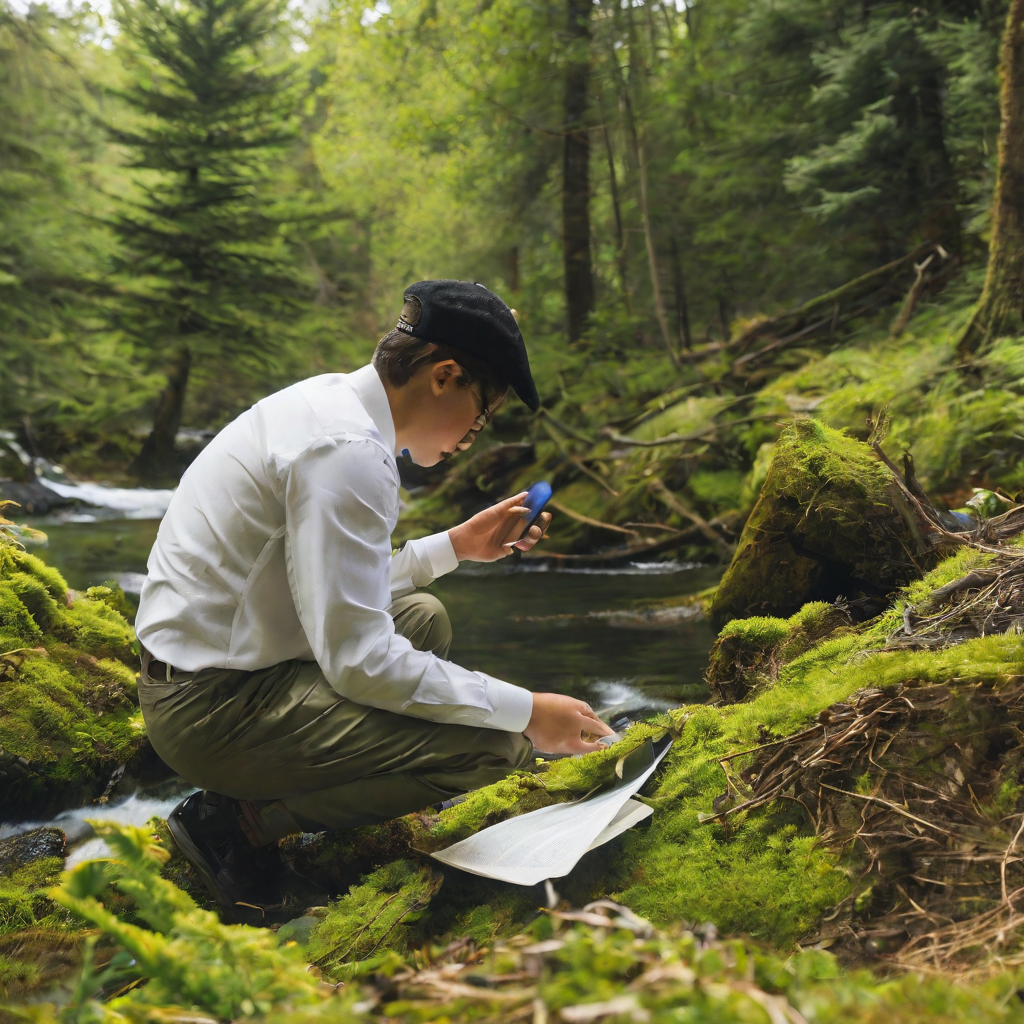
\includegraphics[width=0.9\textwidth]{fig3_1}
\end{columns}
\end{frame}
%%%%%%%%


%%%%%%%%
\section{¿Cuales son las dimensiones de la elecci\'on de un problema?}
\begin{frame}{Las dos dimensiones de la escogencia de un problema}
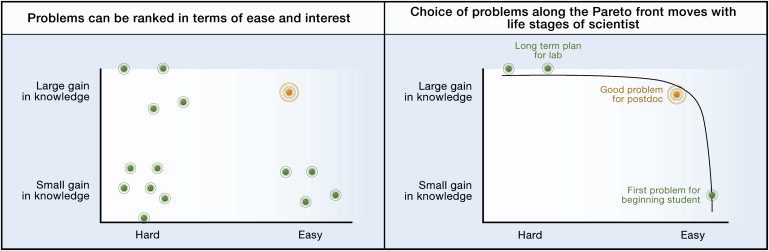
\includegraphics[width=\textwidth]{fig3_2}
\begin{itemize}
\item \alert{Es recomendable abordar problemas realizables y con un alto impacto (cuadrante superior derecho)}
\item El tipo de problema depende del nivel de experiencia/formaci\'on del investigador.
\end{itemize}
\end{frame}

\begin{frame}{Las dos dimensiones de la escogencia de un problema}
\begin{itemize}
\item El nivel de inter\'es de una idea es algo subjetivo.
\item El inter\'es puede ser relativo a mi entorno (E.j. grupo de invetigaci\'on, departamento).
\item \alert{¿Es interesante para m\'i? En el mediano plazo esto es m\'as importante.}
\begin{itemize}
\item Si yo fuera la \'unica persona en la tierra ¿cual de estos problemas escoger\'ia?
\item Ideas que son recurrentes
\item ¿Como se siente al describir el problema?
\end{itemize}
\end{itemize}
\centering
\alert{Entre m\'as interesado este en su idea, m\'as probabilidades de que su audiencia muestre inter\'es por esta.}
\end{frame}
%%%%%%%%

%%%%%%%%
\section{¿Como encontrar una idea de investigaci\'on o profundizaci\'on?}

\begin{frame}{I. Listar los temas de inter\'es}
\begin{enumerate}
\item[1] \emph{Listar aspectos de la vida aparte de alg\'un inter\'es acad\'emico}: Ej. hobbies, pasiones, inclinaciones pol\'iticas,etc. Explicar porque le interesan cada una de ellas.
\item[2] \emph{Listar \'areas en las que es experto o habilidades que tenga}: Ej. cocinando, tocando guitarra, jugando futbol, idiomas, etc.
\item[3] \emph{Listar disciplinas o \'areas del conocimiento en las que se desenpe\~na}: Ej. Ingenier\'ias, Geociencias, etc. Proporcionar dos razones porque esta interesado y que no le gusta de esta.
\item[4] \emph{Listar todos tus temas acad\'emicos de inter\'es}: Ej. modelaci\'on hidrolgica, cambio clim\'atico, geomorfolog\'ia, calidad del agua, hidrodin\'amica, etc. 
\item[5] \emph{Listar el art\'iculo o libro  acad\'emico que m\'as ha influenciado en su formaci\'on}: Sin buscar en Internet, solo recordando. Ej. 'Una breve historia del tiempo' por Stephen Hawking. Escribir por que es importante.  
\end{enumerate}
\end{frame}

\begin{frame}{I. Listar los temas de inter\'es}
\begin{enumerate}
\item[6] \emph{Listar las teor\'ias acad\'emicas que encuentre m\'as interesantes}: Usando uso de la memor\'ia, \'unicamente. Ej. leyes de Newton, leyes de la termodin\'amica, c\'alculo diferencial, etc. 
\item[7] \emph{Listar noticias o post en Internet que recientemente lo hayan impactado}: Ej. guerra entre Israel y Palestina, record m\'aximo de temperaturas en el mundo, deforestaci\'on en la Amazonia, etc.  
\end{enumerate}
\end{frame}


\begin{frame}{II. Encontrar relaciones entre temas de inter\'es}
Esto se realiza para:
\begin{itemize}
\item Encontrar temas de investigaci\'on que le interesen. Ej. es Ingeniero Civil y le impact\'o una noticia sobre la deforestaci\'on en la Amazon\'ia; tiene habilidades en programaci\'on y quisieras modelar los efectos de la deforestaci\'on en la evapotranspiraci\'on en la Amazon\'ia.
\item Encontrar temas de inter\'es que sean acordes usted. Muchas veces existen temas interesantes pero nuestras habilidades limitan su desarrollo. Ej. siente inter\'es en la formaci\'on de rios y su evoluci\'on pero no me gusta el trabajo de campo y tengo pocas habilidades para construcci\'on de equipos. 
\end{itemize}
\centering
Una fuerte alineaci\'on entre su disciplina, sus habilidades y su inter\'es es clave para encontrar un tema.
\end{frame}

\begin{frame}{III. Indentificar libros y revistas claves}
\begin{itemize}
\item Conocer las controversias o temas m\'as "de moda" en su campo y en que revistas se publican. 
\item Para entender un tema o idea, es fundamental ¡leer mucho!, principalmente, art\'iculos cient\'ificos.
\item Determinar las principales fuentes de informaci\'on: top 5 de las revistas en el campo de inter\'es.
\item Crear una base de datos con referencias bibliogr\'aficas. 
\end{itemize}
\end{frame}

\begin{frame}{IV. Leer art\'iculos relevantes en las revistas principales}
Para las revistas en el top 5, revisar art\'iculos de  inter\'es en los \'ultimos 5 a\~nos de la siguiente manera:
\begin{enumerate}
\item Leer el titulo de cada art\'iculo. Haga una lista de 5 temas recurrentes en los t\'itulos.
\item Leer el abstract de los art\'iculos. Haga un listado de las 5 metodolog\'ias y problemas m\'as comunes. 
\item Determinar cuales problemas y temas encontrados son de su inter\'es.
\item Algunas veces existen temas controversiales y puede ser recomendable contactar al autor para comentar el inter\'es. 
\item De acuerdo con los temas encontrados, escoger los 5 art\'iculos m\'as interesantes y leerlos completamente. Leer "the most cited", "the most downloaded". Extraer el argumento, ¿que encontraron?
\end{enumerate}
\end{frame}


\begin{frame}{V. Brainstorm ideas y argumentos}
De acuerdo con la lectura realizada:
\begin{enumerate}
\item Escribir 10 posibles ideas de investigaci\'on o profundizaci\'on.
\item Escribir estas ideas como preguntas o t\'esis de investigaci\'on.
\item No se preocupe si la idea ya ha sido desarrollada anteriormente.
\item Recuerda que la mejor idea no resulta de manera inmediata, es un proceso gradual.
\end{enumerate}
\end{frame}

%%%%%%%%
\section{Probar las ideas}
\begin{frame}{I. Consultar con profesores acerca de sus ideas y argumentos}
Con base en la lectura realizada:
\begin{enumerate}
\item Contactar tres profesores que pueden tener inter\'es en sus ideas.
\item En 15 minutos exponer las ideas que encontr\'o. Aclarar que son ideas insipientes y que quiere tener su opini\'on.
\item Comunicarle a los profesores que sus respuestas pueden ser: Ej. ¡interesante!, no estoy seguro, ya se hizo, etc
\item Preguntarles cual de las ideas expuestas suena m\'as interesante.
\item No olvidar tomar notas. 
\end{enumerate}
\centering
\alert{No olvide que la idea debe convencerlo a usted, su tutor solo debe estar deacuerdo}
\end{frame}

\begin{frame}{II. Crear argumentos}
Con base en lo anterior:
\begin{itemize}
\item Escoge las ideas que m\'as le interesan.
\item Con base en las ideas, construir argumentos, hip\'otesis y/o preguntas de investigaci\'on en torno a ellas. 
\item Juegue con las ideas, cree met\'aforas entorno a ellas para entender m\'as facilmente el problema.
\item Cree mapas, figuras, dibujos con base en una idea para visualizarla mejor.
\end{itemize}
\end{frame}

\begin{frame}{III. Revisar la literatura}
Revisar referencias de forma r\'apida de la siguiente manera:
\begin{itemize}
\item Revise si las ideas han sido publicadas.
\item Identificar lo que se ha investigado acerca de ellas y que autores lo han hecho.
\item Determinar si se ha dicho mucho o poco respecto a una idea. Recuerde que es f\'acil extender el trabajo de otros.
\item El objeto de esto es determinar si existen traslapos o similitudes con sus argumentos que impiden desarrollar la idea.
\end{itemize}
\end{frame}

\begin{frame}{IV. Revisar metodolog\'ias}
\begin{itemize}
\item Ninguna idea puede ser desarrollada si no se tiene el m\'etodo adecuado. 
\item Identificar en la literatura los m\'etodos usados para desarrollar ideas similares.
\item Determinar que nuevos conocimientos requiero para desarrollar mi idea. Ej. estad\'istica, m\'etodos num\'ericos, electr\'onica, etc.
\end{itemize}
\end{frame}

%%%%%%%%

\begin{frame}{Dificultades comunes en la escogencia del problema}
\begin{itemize}
\item Escoger el primer problema que venga a la mente.
\item Toma tiempo escoger un problema, por eso es recomentable escoger varios hasta llegar al indicado.
\item Muchas veces, existen restricciones de financiaci\'on y tiempo que requieren una escogencia r\'apida.
\item Para escoger un buen problema, debemos vernos reflejados en nuestra propia visi\'on del mundo. 
% techniques or logical proof, basic understanding or applied work, visual aesthetics or abstract ideas.
\end{itemize}
\centering
\alert{Si podemos expresarnos a trav\'es de nuestro proyecto, el trabajo se convierte en algo agradable y que fluye facilmente.}
\end{frame}
%%%%%%%%

%%%%%%%%
\section{Argumento, hip\'otesis o pregunta de investigaci\'on}
\begin{frame}{Definici\'on de argumento}
Argumento = hip\'otesis = pregunta de investigaci\'on
\begin{exampleblock}
Es una \'unica idea significante expresada en dos o tres frases alrededor de la cual su proyecto o trabajo es desarrollado y soportado en evidencias.
\end{exampleblock}
\begin{itemize}
\item La intenci\'on de un argumento es convencer al lector mediante la proporci\'on de cierta evidencia.
\item Un argumento es la respuesta a una pregunta de investigaci\'on o la confirmaci\'on de una hip\'otesis.
\item Busca respuesta a trav\'es del intercambio de ideas. Es una manera de pensar en un problema. 
\end{itemize}
\end{frame}

\begin{frame}{¿Como desarrollar un argumento?}
\begin{exampleblock}{Posusta's template}
\begin{enumerate}
\item Frase general opuesta a la idea principal (Ej. Apesar de ...).
\item Frases acerca de la idea principal o t\'esis (Ej. sin embargo, ...).
\item Frases que muestren la evidencia y ejemplos (Ej. Porque ....).
\end{enumerate}
\end{exampleblock}
\begin{exampleblock}{Simpson's template}
Observando $x$, podemos ver $y$, la cual muchos no ven, y esto es importante porque $z$.
\end{exampleblock}
\end{frame}

\begin{frame}{¿Como desarrollar un argumento?}
\begin{exampleblock}{Belcher's template}
\begin{enumerate}
\item El problema. Lo que otros autores discuten, debaten, asumen, ignoran, etc.
\item En relaci\'on con el problema, yo veo que ... (E.j. oposci\'on, vacio, estoy deacuerdo, etc)
\item La evidencia. Basado en mi estudio, investigaci\'on, previas investigaciones, an\'alisis de la bibliograf\'ia, etc.
\end{enumerate}
\end{exampleblock}
\end{frame}

\begin{frame}{Esquematizar mi argumento}
\begin{itemize}
\item Mapas conceptuales que representen el argumento.
\item Esquema de un argumento que utilice palabras claves, dibujando flechas que conecten palabras.
\item Crear un historieta alrededor del argumento con personajes y un escenario.
\end{itemize}
\end{frame}

\begin{frame}{¿Como fortalecer mi argumento?}
\begin{itemize}
\item Usar contra-argumentos para modificar o afinar un argumento.
\item No estigmatizar autores que se oponen a un argumento.
\item Muchas veces un argumento fuerte consiste en demostrar que el otro esta mal, y principalmente, que yo estoy en lo correcto. 
\item Las evidencias, incluso si debilitan mi argumento, hacen este, al final, m\'as fuerte.
\end{itemize}
\end{frame}
%%%%%%%%


%%%%%%%%
\section{¿Que pasa desp\'ues de escoger el problema?}
\begin{frame}{¿Que pasa despu\'es de escoger el problema?}
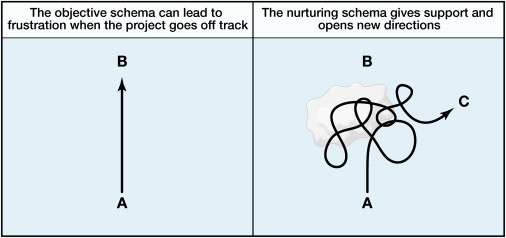
\includegraphics[width=\textwidth]{fig3_3}
\end{frame}

\begin{frame}{¿Que pasa desp\'ues de escoger el problema?}
\begin{itemize}
\item El esquema objetivo puede llevar a depresi\'on y desiluci\'on ante alg\'un traspi\'es o dificultad.
\item El esquema de "nutrir" refleja m\'as lo que es un proyecto. El proyecto va evolucionando a trav\'es de cambios de direcci\'on y sentido. 
\begin{itemize}
\item Un cambio de destino surge porque es m\'as interesante que el destino inicial.
\item Este movimiento, que puede parecer err\'atico, es parte integral de la realizaci\'on del proyecto. 
\item El trabajo de un mentor es guiar al estudiante en aquellos momentos de confusi\'on.
\end{itemize}
\end{itemize}
\centering
\alert{Navegar en lo desconocido requiere coraje; ver y conocer aspectos diferentes a nuestras expectativas}.
\end{frame}
%%%%%%%%



%%%%%%%% %\begin{frame} [allowframebreaks]\frametitle{References}
%        \bibliographystyle{apalike}
%        \bibliography{bibfile}
%\end{frame}

\end{document}

